\documentclass{article}

\usepackage[margin=1in]{geometry}
\usepackage{amsfonts, amsmath}
\usepackage{graphicx}

\newcommand{\R}{\mathbb{R}}

\title{Random Walks on Simple Two-Dimensional Manifolds}
\author{Tom Eichlersmith \\ Art Guetter (adv)}

\begin{document}
	
\maketitle

\section{Introduction and Background}
	For us to be capable of exploring the central problem explained later in this paper, we must develop machinery in order to replicate the intuitive notion of a walk on different surfaces.
	If we are able to determine what a ``step" is on each of our surfaces, then a ``walk" is simply a string of steps connected end-to-end.
	We define a ``step" on a surface as the movement to a point relatively near-by along the shortest path.
	In order to determine this shortest path (as well as the direction the movement is taken), we require calculational tools from differential geometry.
	Most of this machinery has been learned from \cite{BanchoffLovett_DiffGeo_2010} (Read it for a more detailed and precise explanation of this material).
	We will begin with a general overview of differential manifolds that are considered to be ``regular" because of their similarity to what we consider to be intuitively smooth.
	
	\subsection{Regular Surfaces}
		The introduction to parametrized surfaces given in \cite{BanchoffLovett_DiffGeo_2010} is most readily adapted to this project because it can be easily implemented in computer programming.
		We construct a surface as a subset of $\R^3$ by considering continuous functions $\mu:U \to V$ where $U \subseteq \R^2$ and $V$ is a subset of the surface --- we call the set of $\mu$ that covers the entire surface in question a \textit{chart}.
		Glossing over the large amount of detail and development that can be extracted from this simple idea of a surface, we apply more restrictions on the surfaces (and their charts) in order to obtain an intuitive "smoothness" on the surface.
		In a sense, these restrictions allow us to consider surfaces that are locally Euclidean and therefore they more closely resemble what we perceive a surface to be (hence the name for this class of surfaces).
		For a surface to be regular, there must exist a chart that has a member $\mu$ covering an open neighborhood around each point of the surface and satisfies the following conditions:
		\begin{enumerate}
			\item Differentiable --- the coordinate functions of $\mu$ in $\R^3$ have continuous partial derivatives for all orders
			\item Homeomorphic --- $\mu$ and its inverse are continuous
			\item Satisfies the Regularity Condition --- The differential of $\mu$ is a one-to-one linear transformation
		\end{enumerate}
		Often, a member of the chart for a regular surface is called a \textit{coordinate patch} because it imposes a homeomorphic relationship between coordinates in $\R^2$ --- represented by $U$ --- onto a "patch" enclosing an open neighborhood on the surface --- represented by $V$.
		When properly constructed, a chart of a regular surface completely characterizes it, and we can calculate all of the properties of the surface we require from the chart.
		Regular surfaces are the only surfaces we will work with in this paper, and by our definition, are embedded in $\R^3$.
		They are the Euclidean plane, $P$; the two-dimensional sphere of radius $r$, $S(r)$; and the two-dimensional, one-hole torus of polar radius $R$ and axial radius $r$, $T(R,r)$.
		For consistency, we impose the restrictions that all radii are larger than zero and the polar radius of the torus is strictly greater than the axial radius of the torus (i.e. $R > r > 0$).
	
	\subsection{Charts}
		For easier program implementation in C\texttt{++}, we are going to define the charts of our focus surfaces to be slightly different from the usual charts of these surfaces.
		This change is made so that the coordinate patches of $S$ and $T$ have the unit square $I^2 \subset \R^2$ as their domain.
		The chart for the Euclidean plane $P$ is the single coordinate patch (the identity patch) $i: \R^2 \to P$ defined by
		$$ i(u,v) = ( u , v , 0 ) $$
		This is clearly the simplest chart.
		The chart for the unit sphere $S$ consists of two (stereographic) coordinate patches, one being $\sigma:\R^2 \to S$
		$$ \sigma(u,v) = \left( \frac{2u}{1+u^2+v^2} , \frac{2v}{1+u^2+v^2} , \frac{-1+u^2+v^2}{1+u^2+v^2} \right) $$
		Practically, the technical need for the other coordinate patch in order to satisfy the requirements of the chart can be ignored when implementing in a computer program because the difficulties arise only at one infinitesimal point (the \textit{north pole} of the sphere).
		Nevertheless, care will be taken in order to avoid the issues arising from being near this point.
		For our specific situation, we will always have the north pole contained inside of the escape region so that the walk never needs to arrive at that point. 
		Finally, the chart for the torus $T(R,r)$ consists of a single coordinate patch $\tau:I^2 \to T(R,r)$ defined by
		$$ \tau(u,v) = ( (R+r\cos(2\pi v))\cos(2\pi u) , (R+r\cos(2\pi v)\sin(2\pi u) , r\sin(2\pi v) ) $$
		We will use these charts whenever speaking of these surfaces for the rest of this paper, and their form will lead to slightly different calculations that what you see in \cite{BanchoffLovett_DiffGeo_2010,Irons_GeodesicsTorus_2005}.
		
	\subsection{Derivation of Geodesic Equations}
		Geodesics are defined as paths on a surface with no acceleration (relative to the surface).
		This is a method of extending the idea of a line on the plane to other surfaces --- done similarly in \cite{Lewis_GeodesicsMathematica_2002}.
		If $\mu$ represents a coordinate patch on a surface $M$ containing a path $\gamma$, then we can formalize this notion of no acceleration relative to the surface by forcing $\gamma''$ to be normal to the surface everywhere.
		Let $\gamma:[0,1] \to M$, then $\gamma$ is a \textit{geodesic} if
		\begin{equation} \label{geodesic_def} \begin{split}
			&\gamma''(t) \cdot \mu_u = 0 \\
			&\gamma''(t) \cdot \mu_v = 0
		\end{split} \end{equation}
		for all $t$.
		We are able to represent $\gamma(t) = \mu( u(t) , v(t) )$ and expand on this definition to find differential equations for the coordinate functions $u$ and $v$.
		First (omitting the explicit writing of $t$ and writing partial derivatives as subscripts),
		\begin{equation*}
			\gamma' = \mu_u u'+\mu_v v'
		\end{equation*}
		And then (using the fact that since $\mu$ is a coordinate chart, we know $\mu_{uv}=\mu_{vu}$)
		\begin{equation*} \begin{split}
			\gamma'' & = (\mu_{uu} u' + \mu_{uv} v')u' + \mu_u u'' + (\mu_{vu} u' + \mu_{vv} v') v' + \mu_v v'' \\
					 & = (u')^2 \mu_{uu} + (v')^2\mu_{vv} + 2u' v'\mu_{uv} + u''\mu_u + v''\mu_v
		\end{split} \end{equation*}
		Now we can put this expression for $\gamma''$ into equation \ref{geodesic_def} to obtain differential equations that the functions $u(t)$ and $v(t)$ must satisfy in order for $\gamma$ to be a geodesic (also using that $\mu_u$ and $\mu_v$ are orthogonal: $\mu_u \cdot \mu_v = 0$)
		\begin{equation} \label{geodesic_work} \begin{split}
			\gamma'' \cdot \mu_u & = (u')^2\mu_u \cdot \mu_{uu} + (v')^2\mu_u \cdot \mu_{vv} + 2u' v'\mu_u \cdot \mu_{uv} + u''\mu_u \cdot \mu_u + v''\mu_u \cdot \mu_v \\
			0 & = (u')^2\mu_u \cdot \mu_{uu} + (v')^2\mu_u \cdot \mu_{vv} + 2u' v'\mu_u \cdot \mu_{uv} + u''\mu_u \cdot \mu_u \\
			\gamma'' \cdot \mu_v & = (u')^2\mu_v \cdot \mu_{uu} + (v')^2\mu_v \cdot \mu_{vv} + 2u' v'\mu_v \cdot \mu_{uv} + u''\mu_v \cdot \mu_u + v''\mu_v \cdot \mu_v \\
			0 & = (u')^2\mu_v \cdot \mu_{uu} + (v')^2\mu_v \cdot \mu_{vv} + 2u' v'\mu_v \cdot \mu_{uv} + v''\mu_v \cdot \mu_v \\
		\end{split} \end{equation}
		Rearranging equation \ref{geodesic_work} will be more useful for us. We can assume $\mu_u \cdot \mu_u \neq 0$  and $\mu_v \cdot \mu_v \neq 0$ because of the conditions on $\mu$ we imposed earlier.
		\begin{equation} \label{geodesic_eqn} \begin{split}
			u'' + \frac{\mu_{uu} \cdot \mu_u}{\mu_u \cdot \mu_u} (u')^2 + \frac{\mu_{vv} \cdot \mu_u}{\mu_u \cdot \mu_u} (v')^2 + 2\frac{\mu_{uv} \cdot \mu_u}{\mu_u \cdot \mu_u} u'v' & = 0 \\
			v'' + \frac{\mu_{uu} \cdot \mu_v}{\mu_v \cdot \mu_v} (u')^2 + \frac{\mu_{vv} \cdot \mu_v}{\mu_v \cdot \mu_v} (v')^2 + 2\frac{\mu_{uv} \cdot \mu_v}{\mu_v \cdot \mu_v} u'v' & = 0 \\
		\end{split} \end{equation}
		In this form we can pick out the Christoffel Symbols (usually defined in reference to the metric) as the coefficients of the derivatives of $u$ and $v$. Specifically,
		\begin{equation}
			\Gamma^i_{jk} = \frac{\mu_{jk} \cdot \mu_i}{\mu_i \cdot \mu_i}
		\end{equation}
		where $i,j,k$ run over $u$ and $v$.
		This "definition" means we can write equation \ref{geodesic_eqn} in tensor notation
		\begin{equation} \label{geodesic_chris}
			\frac{d^2 x^i}{dt^2} + \sum_{j,k = 1}^2 \Gamma^i_{jk} \frac{d x^j}{dt} \frac{dx^k}{dt} = 0
		\end{equation}
		In \cite{BanchoffLovett_DiffGeo_2010}, equation \ref{geodesic_chris} uses $s$ as the independent variable because these equations produce a geodesic that is parametrized by arc length (has unit speed) when the proper initial conditions are given to it.
		Specifically, if the initial direction vector has unit magnitude, then the resulting solution will have unit speed (and therefore be parametrized by arc length).
		
	\subsection{Christoffel Symbols}
		The computer implementation of steps along geodesics uses equation \ref{geodesic_chris}, so we can completely characterize the geodesics (and therefore walk on the surfaces) by calculating the Christoffel symbols.
		Below are the calculations producing the symbols for each of the coordinate patches from above generated using the CAS \textit{Mathematica}.
		
		The symbols calculated from $i$ are quickly obtained.
		Since all of the symbols contain second partial derivatives and $i$ only has linear orders of $u$ or $v$, all of the symbols on the plane are zero.
		\begin{equation}
			\begin{array}{lr}
				\left(\Gamma^{u}_{ij}\right) = \left( \begin{array}{cc}
					0 & 0 \\
					0 & 0
				\end{array} \right) &
				\left(\Gamma^{v}_{ij}\right) = \left( \begin{array}{cc}
					0 & 0 \\
					0 & 0
				\end{array} \right)
			\end{array}
		\end{equation}
		
		The coordinate patch that's a member of the chart of $S$ (and that we will be using for calculations) has the symbols
		\begin{equation}
			\begin{array}{lr}
			\left(\Gamma^{u}_{ij}\right) = \left( \begin{array}{cc}
					-\frac{2u}{1+u^2+v^2} & -\frac{2v}{1+u^2+v^2} \\
					-\frac{2v}{1+u^2+v^2} & \frac{2u}{1+u^2+v^2}
				\end{array} \right) &
			\left(\Gamma^{v}_{ij}\right) = \left( \begin{array}{cc}
					\frac{2v}{1+u^2+v^2} & -\frac{2u}{1+u^2+v^2} \\
					-\frac{2u}{1+u^2+v^2} & -\frac{2v}{1+u^2+v^2}
				\end{array} \right)
			\end{array}
		\end{equation}
		
		The coordinate patch we are using for the torus covers the entire surface with no problematic points (as long as domain wrapping is kept consistent).
		The Christoffel symbols for $\tau$ are
		\begin{equation}
			\begin{array}{lr}
				\left(\Gamma^{u}_{ij}\right) = \left( \begin{array}{cc}
					0 & -\frac{2\pi r\sin(2\pi v)}{R+r\cos(2\pi v)} \\
					-\frac{2\pi r\sin(2\pi v)}{R+r\cos(2\pi v)} & 0
				\end{array} \right) &
				\left(\Gamma^{v}_{ij}\right) = \left( \begin{array}{cc}
					\frac{2\pi}{r}\sin(2\pi v)(R+r\cos(2\pi v)) & 0 \\
					0 & 0
				\end{array} \right)
			\end{array}
		\end{equation}
	
\section{Random Walks}
	Now that we have all of the tools necessary to take steps on each of our three surfaces, we are able to walk on them.
	The implementation of these walks is in C\texttt{++} using an application of the standard Runge-Kutta method to numerically solve the geodesic equations in steps.
	Once we are able to take a single step in any direction and from any point on the surface, we are able to randomly walk on the surface.
	By \textit{random walk} (or simply \textit{walk}), we mean that the direction of each step is randomly chosen uniformly.
	A general structure to walk on a given surface is constructed in the package \texttt{MOSEY} where one can define a surface by its Christoffel symbols (\texttt{MOSEY::CurveTensor}) and how its coordinates connect across domain edges (\texttt{MOSEY::CoordinateWrappers}).
	The walks are done in the coordinate space and then output to a \texttt{csv}-file in a format depending on the situation --- for example, the walk distances are output with respect to latitudes when walking on the sphere.
	
	For each situation, we define an \textit{escape region} where a walk ends if entered.
	These escape regions allow us to be able to study the behavior of walks on different surfaces by analyzing the ``distance" different points on a surface are from escaping.
	We define a walk's \textit{length} to be the sum of the steps it has to take for it to enter the escape region.
	This leads to general questions that can be explored using the package \texttt{MOSEY}.
	How are the walk lengths and escape regions related?
	How much of an impact does the surface the walk is on have?
	Does the size of the escape region (relative to the surface) have a large effect?
	
	\subsection{Stepping Method}
		The Runge-Kutta method is a process to approximate first order differential equations.
		We will be using the standard, fourth order Runge-Kutta method (RK4) that will be outlined for our specific problem below.
		First, we must transform our two second order geodesic equations \ref{geodesic_chris} into a system of first order differential equations so that we are able to apply the RK4 method.
		
		We begin by expanding \ref{geodesic_chris} and using $u$ and $v$ instead of $x^1$ and $x^2$.
		\begin{equation} \label{geodesic_expansion} \begin{split} 
			\frac{d^2u}{dt^2} & = -\Gamma^u_{uu}\left(\frac{du}{dt}\right)^2-2\Gamma^u_{uv}\frac{du}{dt}\frac{dv}{dt}-\Gamma^u_{vv}\left(\frac{dv}{dt}\right)^2 \\
			\frac{d^2v}{dt^2} & = -\Gamma^v_{uu}\left(\frac{du}{dt}\right)^2-2\Gamma^v_{uv}\frac{du}{dt}\frac{dv}{dt}-\Gamma^v_{vv}\left(\frac{dv}{dt}\right)^2 \\
		\end{split} \end{equation}
		Define the first derivatives of $u$ and $v$ as their own variables
		\begin{equation*} \begin{array}{cc}
			p = \frac{du}{dt} & q = \frac{dv}{dt}
		\end{array} \end{equation*}
		Then \ref{geodesic_expansion} becomes
		\begin{equation} \begin{split}
			\frac{du}{dt} & = p \\
			\frac{dv}{dt} & = q \\
			\frac{dp}{dt} & = -\Gamma^u_{uu}p^2-2\Gamma^u_{uv}pq-\Gamma^u_{vv}q^2 \\
			\frac{dq}{dt} & = -\Gamma^v_{uu}p^2-2\Gamma^v_{uv}pq-\Gamma^v_{vv}q^2 \\
		\end{split} \end{equation}
		This is a system of first order differential equations, so we can adapt RK4 to numerically solve it.
		
		Define $y = \langle u , v , p , q \rangle$.
		Suppose $(u_0,v_0)$ is the point we wish to step from and we are moving at an angle $\theta$ relative to the positive $u$ axis (at that point).
		Then the initial vector is $y_0 = \langle u_0 , v_0 , \cos(\theta) , \sin(\theta) \rangle$.
		This begins the geodesic with unit speed, meaning that it is parametrized by arc length, so if we wish to step a distance $h$, we numerically solve the initial value problem
		\begin{equation} \label{RK4_imp} \begin{split}
			\frac{dy}{dt} & = F(y) = \langle p , q , -\Gamma^u_{uu}p^2-2\Gamma^u_{uv}pq-\Gamma^u_{vv}q^2 , -\Gamma^v_{uu}p^2-2\Gamma^v_{uv}pq-\Gamma^v_{vv}q^2 \rangle \\
			y(0) & = y_0
		\end{split} \end{equation}
		until $t = h$.
		Let $N$ be the number of iterations of the RK4 method we will use to approximate \ref{RK4_imp}.
		Define $\delta = h/N$, then we write our approximation scheme below.
		\begin{equation} \label{RK4_alg} \begin{split}
			& y \gets y_0 \\
			& \textit{loop } N \textit{ times:} \\
			& \quad k_1 \gets F(y) \\
			& \quad k_2 \gets F\left(y+(\delta/2)k_1\right) \\
			& \quad k_3 \gets F\left(y+(\delta/2)k_2\right) \\
			& \quad k_4 \gets F\left(y + \delta k_3\right) \\
			& \quad y \gets y+(\delta/6)(k_1+2k_2+2k_3+k_4)
		\end{split} \end{equation}
		When implemented correctly, the loop exits with $y$ containing an approximate value for $u$, $v$, $p$, and $q$ a distance $h$ away from $(u_0, v_0)$ on the surface.
		This method is constructed in the \texttt{MOSEY::Stepper} class.
		
	\subsection{Optimizations}
		In order for the walks on the different surfaces to be efficiently studied, some situations admit specific optimizations, saving computing time.
		We are not claiming these processes to be perfectly optimized (read \cite{Redfield_NumericalGeodesics_2007} for a more detailed exploration of efficient numerical solutions to the geodesic equations), but we wish to explain the methods we have used to make the simulation of walks more efficient.
		
		The first (and most widely applicable) optimization is recording every step of a random walk as if it was the first step of the walk following it.
		This allows for several walks starting from different initial positions to be acquired at once.
		We are able to use this data because steps are independent of their predecessors.
		
		Walks on the plane offer the massive simplification of having all zero Christoffel symbols.
		In order to take a step of length $h$ at an angle $\theta$ from the positive $u$-axis, we could simply add $(h\cos(\theta), h\sin(\theta))$ to the initial point.
		We do not do this because we would like uniformity across the code package.
		However, using RK4 with the number of iterations $N = 1$ produces the exact same result algebraically.
		Due to the limited precision of numbers in computers, this equality is not perfect; nevertheless, it produces a result that only differs from the exact result due to inherent truncation errors in the computer (which implementing the exact result would suffer from as well).
		Therefore, when the class \texttt{MOSEY::Stepper} is configured to take a step on $P$, the number of iterations used in RK4 is set to one (overriding any user specifications).
		This avoids unnecessary calculations from additional loops that would not produce a more accurate result.
		
		The two-dimensional sphere is also incredibly symmetrical.
		In this specific situation, the escape regions are generally circles with centers at one of the poles.
		Because of the symmetry around the axis of the sphere, we are able to only consider latitude when analyzing how the walk distance changes depending on the starting location.
		We calculate the latitude $\phi$ of $\sigma(u,v)$ by
		\begin{equation*}
			\phi = \arctan\left(\frac{1}{u^2+v^2}\right)
		\end{equation*}
		This simplification will not help the walks themselves be simulated more efficiently; nevertheless, it will allow for the analysis of the data gathered from the walks be simplified --- making it one-dimensional instead of two.
		
		Due to the inherently large amount of noise generated by collecting data in a purely pseudo-random fashion, the general trends that we expect to appear only arise after several hundred (if not more) walks.
		Since each walk is hundreds or even thousands of steps (and each step is treated as its own data point), we are required to have millions of data points collected for each manifold-escape region pair.
		This amount of data leads to an inability to process it all, so we have chosen to compress the data into summary files that are at most one hundred thousand data points.
		The raw data is still stored; nevertheless, these summary files are valuable to construction of plots that would crash under the weight of millions of points.
		The compression method is binning the data into small bins and determining the mean for each bin.
		This procedure substitutes one data point for a few thousand, which quickens analysis and plotting.

\section{Numeric Solution}

\section{Results}
	\subsection{Plane}
		\subsubsection{Ring}
		\subsubsection{Circular Walls}
	\subsection{Sphere}
		\begin{figure}[h]
			\centering
			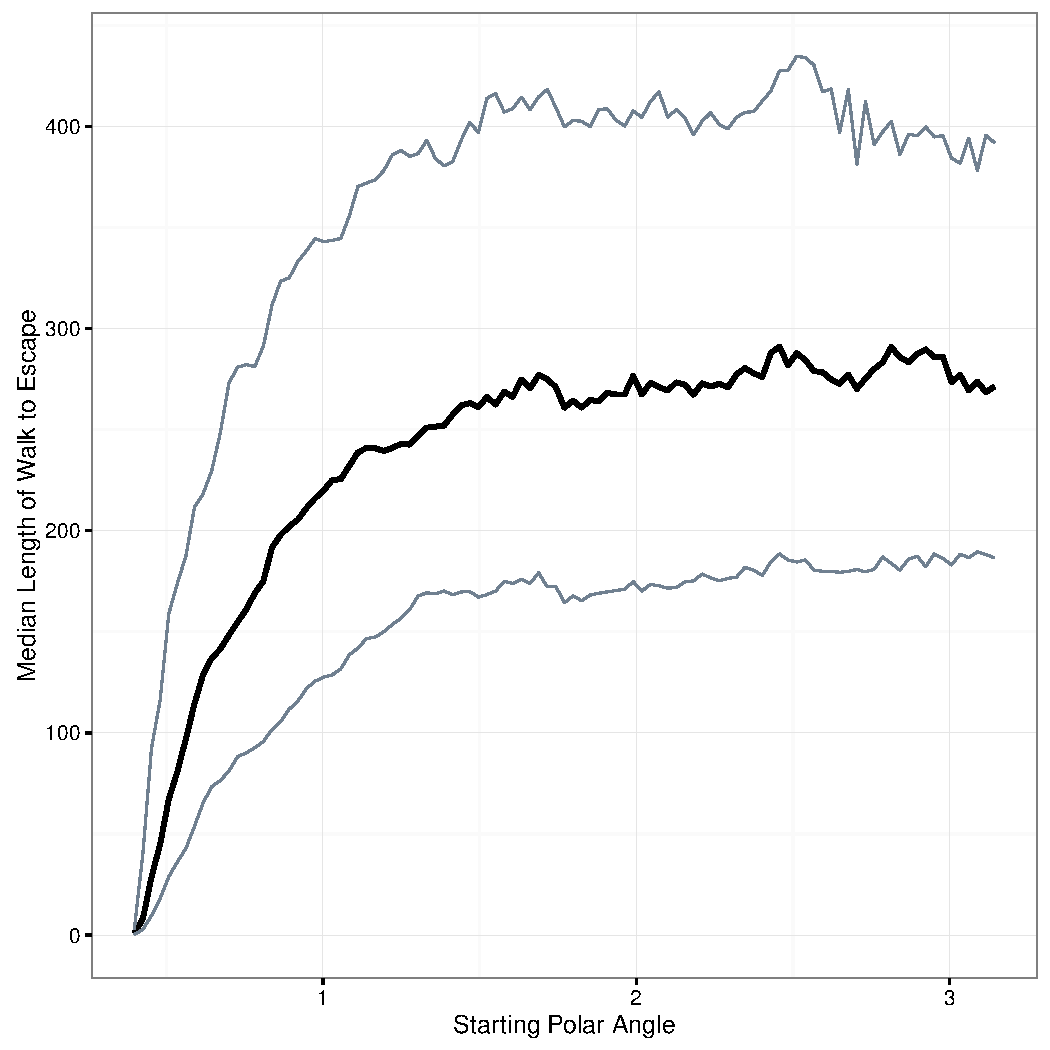
\includegraphics[width=0.5\textwidth]{images/ExampleSphereL04.pdf}
			\caption{Example data plot from the sphere with the escape region beginning at latitude $0.4$ --- Red is the raw data and blue is the compressed means.}
		\end{figure}
	\subsection{Overall Package}
	
\bibliographystyle{plain}
\bibliography{../../References/References_MathDHP_201718}

\end{document}